% !TEX root = ../Monografia.tex

\subsection{Fase 2 – Levantamento de Requisitos e Especificação}

A segunda fase envolveu o levantamento e a análise dos requisitos funcionais e não funcionais do sistema, de forma a alinhar a proposta às necessidades práticas de desenvolvedores Flutter.
Seguindo o modelo sugerido por Sommerville~\cite{sommerville2019software}, o processo de elicitação de requisitos considerou aspectos de usabilidade, integração, portabilidade e impacto sobre o desempenho.

\subsubsection{Requisitos Funcionais}

Os requisitos funcionais definem as operações que o sistema deve realizar. Entre os principais, destacam-se:

\begin{itemize}
  \item RF1 – Coletar métricas de desempenho em tempo real, incluindo FPS, reconstruções de widgets, uso de memória e duração de quadros;
  \item RF2 – Processar e correlacionar as métricas coletadas, identificando padrões de degradação de desempenho;
  \item RF3 – Gerar recomendações heurísticas de otimização baseadas em boas práticas do ecossistema Flutter;
  \item RF4 – Exibir métricas e recomendações em um painel visual integrado ao aplicativo;
  \item RF5 – Permitir a simulação de cenários de carga e coleta sob condições controladas.
\end{itemize}

\subsubsection{Requisitos Não Funcionais}

Os requisitos não funcionais descrevem as propriedades de qualidade esperadas do sistema, como desempenho, compatibilidade e manutenibilidade (Pressman e Maxim~\cite{pressman2020engenharia}):

\begin{itemize}
  \item RNF1 – O sistema deve operar majoritariamente em Dart, utilizando \textit{platform channels} apenas para métricas dependentes do sistema operacional, como CPU e bateria;
  \item RNF2 – O coletor deve introduzir um \textit{overhead} máximo de 5\% sobre o tempo médio de renderização da aplicação monitorada;
  \item RNF3 – A interface do painel deve manter atualização fluida e responsiva, com taxa mínima de 50 FPS em dispositivos de médio desempenho;
  \item RNF4 – A arquitetura deve seguir princípios de modularidade e separação de responsabilidades (Martin~\cite{martin2018clean});
  \item RNF5 – O sistema deve permitir reuso e extensão, facilitando a integração de novos tipos de métricas ou heurísticas adicionais.
\end{itemize}

\noindent\textbf{Nota sobre limites de overhead.}
O RNF2 estabelece um valor máximo de \textbf{5\%} de overhead aceitável
para garantir que o coletor não comprometa o desempenho perceptível da
aplicação. Entretanto, o valor de \textbf{3\%} citado nos resultados esperados
refere-se a uma \textit{meta de projeto}, mais conservadora, adotada
para assegurar margem de segurança entre a operação real e o limite
permitido pelos requisitos não funcionais.

\subsection{Fase 3 – Projeto e Implementação do Pacote}

Nesta etapa, foram definidas as estruturas de software, as tecnologias empregadas e o fluxo de integração entre módulos. O projeto adotou a \textbf{Clean Architecture} proposta por Martin~\cite{martin2018clean}, visando garantir independência entre camadas e testabilidade.



\subsubsection{Modelagem e Arquitetura de Software}

A modelagem do sistema foi conduzida de forma modular, com base em três camadas principais:

\begin{enumerate}
  \item \textbf{Data:} responsável pela coleta e serialização de métricas;
  \item \textbf{Domain:} núcleo da lógica de negócio, contendo entidades, repositórios e casos de uso;
  \item \textbf{Presentation:} interface de usuário e controle de estado.
\end{enumerate}

Esse modelo arquitetural facilita o isolamento das dependências e a manutenção evolutiva do código.

A Figura~\ref{fig:architecture} ilustra a arquitetura local adotada no pacote.
Ela organiza o \collectorFlutter{} em coleta, telemetria, análise, recomendações e visualização integrada.

\begin{figure}[H]
  \centering
  
\includegraphics[width=0.95\textwidth]{arquitetura_fluxo_collector.png}
  \caption{Arquitetura local e fluxo de dados do pacote \collectorFlutter{}: coleta, análise, recomendação e apresentação no painel integrado.}
  \label{fig:architecture}
\end{figure}

A modelagem de entidades e casos de uso foi organizada de forma a manter as regras de análise separadas dos detalhes de coleta e apresentação.

\subsubsection{Tecnologias e Ferramentas Utilizadas}

O ambiente de desenvolvimento foi configurado com as seguintes ferramentas e tecnologias:
\begin{itemize}
  \item \textbf{Flutter SDK} (versão 3.22 ou superior) e \textbf{Dart SDK};
  \item \textbf{Android Studio} e \textbf{Visual Studio Code} como IDEs principais;
  \item \textbf{Bibliotecas:} \texttt{flutter\_bloc} para controle de estado, \texttt{fl\_chart} para geração de gráficos e \texttt{vm\_service} para instrumentação de métricas internas;
  \item \textbf{Controle de versão:} GitHub para versionamento e reprodutibilidade científica (Wohlin \textit{et al.}~\cite{wohlin2012}).
\end{itemize}

\subsubsection{Integração dos Módulos e Testes Iniciais}

Após a implementação individual dos módulos, foi conduzida uma fase de integração incremental, conforme orientam Sommerville~\cite{sommerville2019software}.
O processo envolveu:
\begin{itemize}
  \item Testes unitários em cada componente da camada \textbf{Data} e \textbf{Domain};
  \item Integração dos módulos via \texttt{StreamController} e \texttt{Bloc};
  \item Validação visual do painel (\textbf{Dashboard}) com dados simulados;
  \item Confronto qualitativo com sinais observados no painel e com leituras complementares obtidas por ADB.
\end{itemize}

\subsection{Fase 4 – Avaliação Experimental e Validação}

A última fase compreendeu o planejamento, execução e análise de cenários controlados com o pacote, visando validar sua operacionalidade, a coerência das métricas coletadas e a pertinência das recomendações heurísticas. A avaliação apresentada neste trabalho tem caráter funcional e qualitativo, delimitado aos cenários e dispositivos descritos nesta metodologia.

\subsubsection{Planejamento dos Cenários}
\subsubsection{Variáveis do Experimento}

Para estruturar os cenários de forma sistemática, foram definidas variáveis observadas e condições de controle, conforme recomendado em experimentação em engenharia de software~\cite{wohlin2012}.

\begin{itemize}

\item \textbf{Condições manipuladas}
\begin{itemize}
\item tipo de cenário de carga (interface, rede, memória ou combinado).
\item acionamento manual das rotinas de simulação no aplicativo de exemplo.
\end{itemize}

\item \textbf{Métricas observadas}
\begin{itemize}
\item FPS médio;
\item tempo médio de renderização de quadros;
\item uso de memória;
\item número de reconstruções de widgets.
\item eventos de rede e recomendações emitidas.
\end{itemize}

\item \textbf{Variáveis de controle}
\begin{itemize}
\item versão do Flutter SDK;
\item modelo do dispositivo utilizado;
\item modo de execução da aplicação (\textit{profile});
\item sequência de acionamento dos cenários.
\end{itemize}

\end{itemize}

O planejamento experimental foi orientado pelas diretrizes de Wohlin \textit{et al.}~\cite{wohlin2012}, contemplando a definição de cenários, variáveis e procedimentos de coleta. As hipóteses foram tratadas como expectativas de funcionamento do pacote:

\begin{itemize}
  \item H1 – O \texttt{collector\_flutter} registra métricas coerentes com os cenários de carga induzidos;
  \item H2 – A coleta não impede a execução interativa do aplicativo de demonstração;
  \item H3 – As recomendações geradas são compatíveis com os sintomas provocados nos cenários.
\end{itemize}

\subsubsection{Execução dos Testes}

Os testes foram conduzidos no aplicativo de exemplo em ambiente Android, sob diferentes tipos de carga. Foram utilizadas variações intencionais de complexidade gráfica, chamadas de rede, alocação de memória e reconstruções de widgets, a fim de provocar gargalos observáveis. Durante as execuções, os sinais exibidos pelo painel foram confrontados qualitativamente com o comportamento esperado dos cenários e com observações em ferramentas oficiais de diagnóstico Android~\cite{android2024}.

\subsubsection{Coleta e Análise de Dados}

A coleta de dados foi realizada de forma automatizada, com as métricas sendo armazenadas em formato JSON e processadas pelo módulo \texttt{Analyzer}.
A análise baseou-se na inspeção dos registros exportados, das mensagens de recomendação e da resposta visual do painel durante os cenários controlados.

Os resultados foram então avaliados segundo os critérios definidos na Seção de \textbf{Critérios de Avaliação}, considerando coerência das métricas, impacto percebido da coleta e pertinência das recomendações.

\subsubsection{Métricas Relacionadas à Eficiência Energética}

Neste trabalho, a eficiência energética foi tratada por meio de \textbf{métricas indiretas}
(\textit{energy proxies}), conforme utilizado em trabalhos sobre estimativa,
perfilamento e diagnóstico energético em aplicações móveis~\cite{hao2013estimating,li2014empirical,hoque2015energy,sun2023energyinefficiency}.
Devido à indisponibilidade de instrumentação física dedicada para medir corrente elétrica, foram observados os seguintes proxies:

\begin{itemize}
    \item uso médio de CPU;
    \item tempo de renderização de quadros;
    \item quantidade de operações de reconstrução;
    \item número de chamadas de rede;
    \item uso de memória.
\end{itemize}

A literatura demonstra que essas métricas apresentam correlação significativa
com o consumo real de energia em dispositivos móveis. A análise energética foi, portanto, inferencial e qualitativa, limitada à observação dos sinais coletados pelo pacote.


\subsubsection{Validação das Recomendações Heurísticas}

A eficácia das recomendações geradas pelo módulo \texttt{Recommender}
foi avaliada verificando se os alertas emitidos correspondiam aos sintomas induzidos em cada cenário controlado:

\begin{itemize}
    \item queda de FPS e aumento de \textit{jank} em cargas de interface;
    \item crescimento de memória durante alocações intensivas;
    \item aumento de eventos e latência em chamadas de rede;
    \item priorização de recomendações quando múltiplos sintomas ocorrem simultaneamente.
\end{itemize}

Essa validação permitiu discutir a pertinência das heurísticas implementadas sem caracterizar um estudo estatístico de eficácia.


% ---------------------------------------------------------------------------------------------------------------------------------------------------------



% ---------------------------------------------------------------------------------------------------------------------------------------------------------
\section{Descrição do Pacote e Arquitetura da Solução}
% ---------------------------------------------------------------------------------------------------------------------------------------------------------

O pacote desenvolvido, denominado \texttt{collector\_flutter}, foi projetado para funcionar de forma totalmente embutida no aplicativo Flutter, realizando a coleta, análise e visualização de métricas de desempenho sem recorrer a servidores externos.
A proposta fundamenta-se na construção de um sistema modular, multiplataforma e de baixo \textit{overhead}, conforme boas práticas de engenharia de software experimental (Wohlin \textit{et al.}~\cite{wohlin2012}; Pressman e Maxim~\cite{pressman2020engenharia}).

\subsection{Concepção e Premissas de Projeto}

A concepção do sistema teve como premissas fundamentais:

\begin{itemize}
  \item Executar majoritariamente em Dart, recorrendo a \textit{platform channels} apenas para métricas dependentes do sistema operacional, como CPU e bateria;
  \item Fornecer medições precisas em tempo real, com impacto mínimo sobre o desempenho do aplicativo monitorado;
  \item Manter arquitetura modular, permitindo substituição ou expansão de componentes;
  \item Adotar interface integrada ao próprio aplicativo, sem uso de ferramentas externas;
  \item Seguir princípios da \textbf{Clean Architecture} (Martin~\cite{martin2018clean}), assegurando separação de responsabilidades e testabilidade.
\end{itemize}

Essas premissas visam garantir a reprodutibilidade científica e a aplicabilidade prática do pacote tanto em ambientes de desenvolvimento quanto em contextos de ensino e pesquisa.

\subsection{Arquitetura Geral do Sistema}

A arquitetura do sistema é organizada em três camadas conceituais \textit{Data}, \textit{Domain} e \textit{Presentation} que interagem de forma desacoplada e síncrona por meio de \texttt{Streams} reativas.
A visão geral dessa organização foi apresentada na Figura~\ref{fig:architecture}, que também explicita o fluxo entre coleta, análise, recomendações e painel visual.

\subsubsection{Camada Data}

A camada \textbf{Data} é responsável pela coleta, persistência e serialização das métricas.
Nela, o módulo \texttt{ResourceCollector} utiliza APIs do Flutter, como \texttt{SchedulerBinding} e \texttt{FrameTiming}, para capturar informações de desempenho, convertendo-as em estruturas JSON processáveis.
Os dados são transmitidos por \texttt{Streams} para as camadas superiores, garantindo atualização contínua e não bloqueante.

\subsubsection{Camada Domain}

A camada \textbf{Domain} implementa os casos de uso e a lógica central do sistema, incluindo os módulos de análise (\texttt{Analyzer}) e recomendação (\texttt{Recommender}).
Ela é responsável por correlacionar as métricas coletadas, identificar gargalos e aplicar heurísticas de otimização baseadas em sintomas recorrentes de degradação, como queda de FPS, aumento de tempo de quadro, crescimento de memória e excesso de chamadas de rede.

\subsubsection{Camada Presentation}

A camada \textbf{Presentation} fornece a interface visual (\texttt{Dashboard}), responsável por exibir métricas, gráficos e recomendações em tempo real.
Sua estrutura é construída sobre o padrão \textit{Bloc/Cubit}, assegurando controle de estado previsível e reatividade imediata na exibição das métricas.

\subsection{Componentes Principais}

O sistema é composto por módulos de coleta, análise, recomendação, apresentação e exportação, que operam de forma integrada e independente.

\subsubsection{Collector}

O módulo \texttt{Collector} é o núcleo de instrumentação do sistema, responsável pela captura de eventos como reconstruções de widgets, tempo de renderização de quadros e uso de memória.
Ele oferece uma API acessível ao desenvolvedor com métodos como \texttt{recordWidget\-Rebuild()}, \texttt{recordNetwork()} e \texttt{recordFrameTiming()}, além de permitir o registro de eventos personalizados.

\subsubsection{Analyzer}

O módulo \texttt{Analyzer} processa as métricas recebidas e detecta padrões que indiquem degradação de desempenho como aumento de tempo de \textit{frame}, quedas de FPS e variações abruptas de reconstruções.
Ele correlaciona dados entre diferentes fontes e envia resultados interpretados ao módulo de recomendação.

\subsubsection{Recommender}

O módulo \texttt{Recommender} interpreta as anomalias detectadas e aplica um conjunto de regras heurísticas baseadas em práticas recomendadas do Flutter.
As recomendações são priorizadas por impacto e apresentadas de forma textual e visual ao desenvolvedor, promovendo a melhoria contínua do aplicativo.

\subsubsection{Dashboard}

O módulo \texttt{Dashboard} constitui o painel visual do sistema, exibindo métricas em tempo real e recomendações automáticas de otimização.
Ele é atualizado dinamicamente a partir de \texttt{Streams} internas e utiliza gráficos, indicadores de status e alertas coloridos para facilitar a interpretação.

\subsubsection{ExportService}

O módulo \texttt{ExportService} permite exportar a sessão de telemetria em JSON e os \textit{timings} de quadros em CSV, ampliando o uso do sistema para contextos de pesquisa e auditoria de desempenho.

\subsection{Interface e Painel de Visualização}

A interface visual foi concebida para proporcionar clareza, responsividade e atualização contínua dos dados, sem prejudicar a experiência do desenvolvedor.
O painel é dividido em áreas funcionais complementares, que permitem análise simultânea e intuitiva das métricas coletadas.

\subsubsection{Área de Métricas}

Exibe os principais indicadores de desempenho como FPS médio, consumo de memória e número de reconstruções de widgets.
Cada indicador é representado por \textbf{cards coloridos} e ícones que sinalizam o estado atual da aplicação: verde (ideal), amarelo (atenção) e vermelho (crítico).

\subsubsection{Área de Recomendações}

Apresenta as sugestões geradas pelo módulo \texttt{Recommender}, priorizadas conforme impacto estimado.
Essas recomendações auxiliam o desenvolvedor a identificar causas potenciais de lentidão e a aplicar boas práticas de otimização no código.

\subsubsection{Gráfico Temporal e Indicadores}

Inclui um gráfico de linha em tempo real, construído com a biblioteca \texttt{fl\_chart}, mostrando a variação temporal do tempo de renderização de quadros.
Esse componente visual é essencial para identificar flutuações de desempenho, travamentos e pontos de gargalo durante a execução.

\subsubsection{Botões de Simulação e Teste}

Disponibilizados na barra inferior do painel, permitem executar cenários artificiais de carga, como:
\begin{itemize}
  \item \texttt{Jank:} simula travamentos intencionais no \textit{main thread};
  \item \texttt{Memória:} aloca objetos grandes para testar consumo e descarte;
  \item \texttt{Rede:} realiza múltiplas chamadas simultâneas;
  \item \texttt{Rebuilds:} força reconstruções sucessivas da árvore de widgets.
\end{itemize}
Esses testes auxiliam na validação experimental do sistema sob diferentes condições de estresse.

A Figura~\ref{fig:prototype_ok} apresenta o painel em uma condição estável, na qual os indicadores permanecem em faixas aceitáveis e as recomendações têm caráter informativo. Essa tela demonstra o estado de referência usado para comparar visualmente as situações de alerta durante os testes.

\begin{figure}[H]
  \centering
  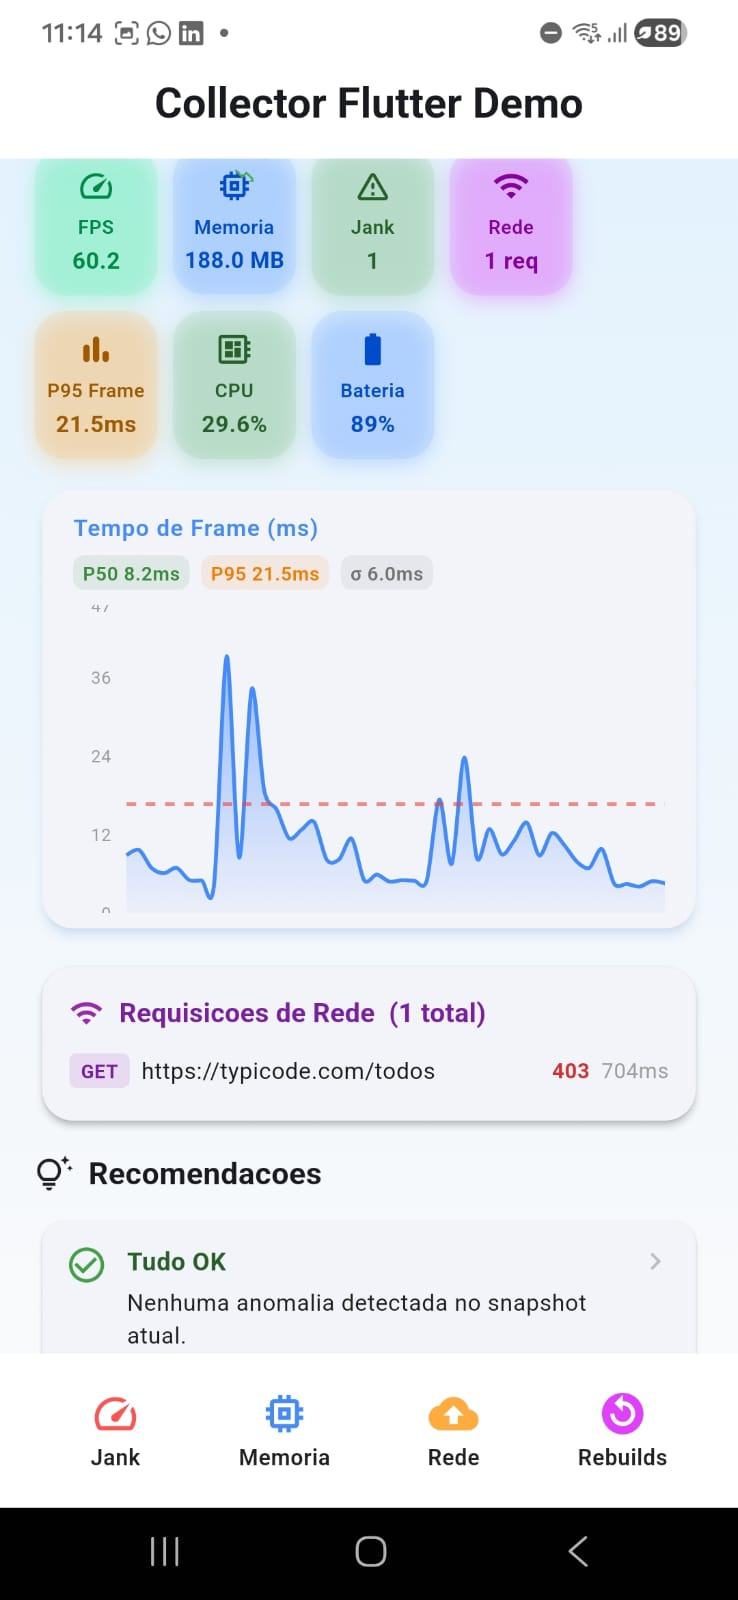
\includegraphics[height=0.8\textwidth]{prototipoquandoestaok.jpeg}
  \caption{Painel do aplicativo em condição de desempenho estável, com indicadores verdes e recomendações informativas.}
  \label{fig:prototype_ok}
\end{figure}

A Figura~\ref{fig:prototype_notok} mostra o comportamento esperado quando há gargalos detectados: os cartões de métricas mudam de cor, o gráfico temporal passa a evidenciar oscilações e as recomendações deixam de ser apenas informativas para orientar possíveis ações de otimização.

\begin{figure}[H]
  \centering
  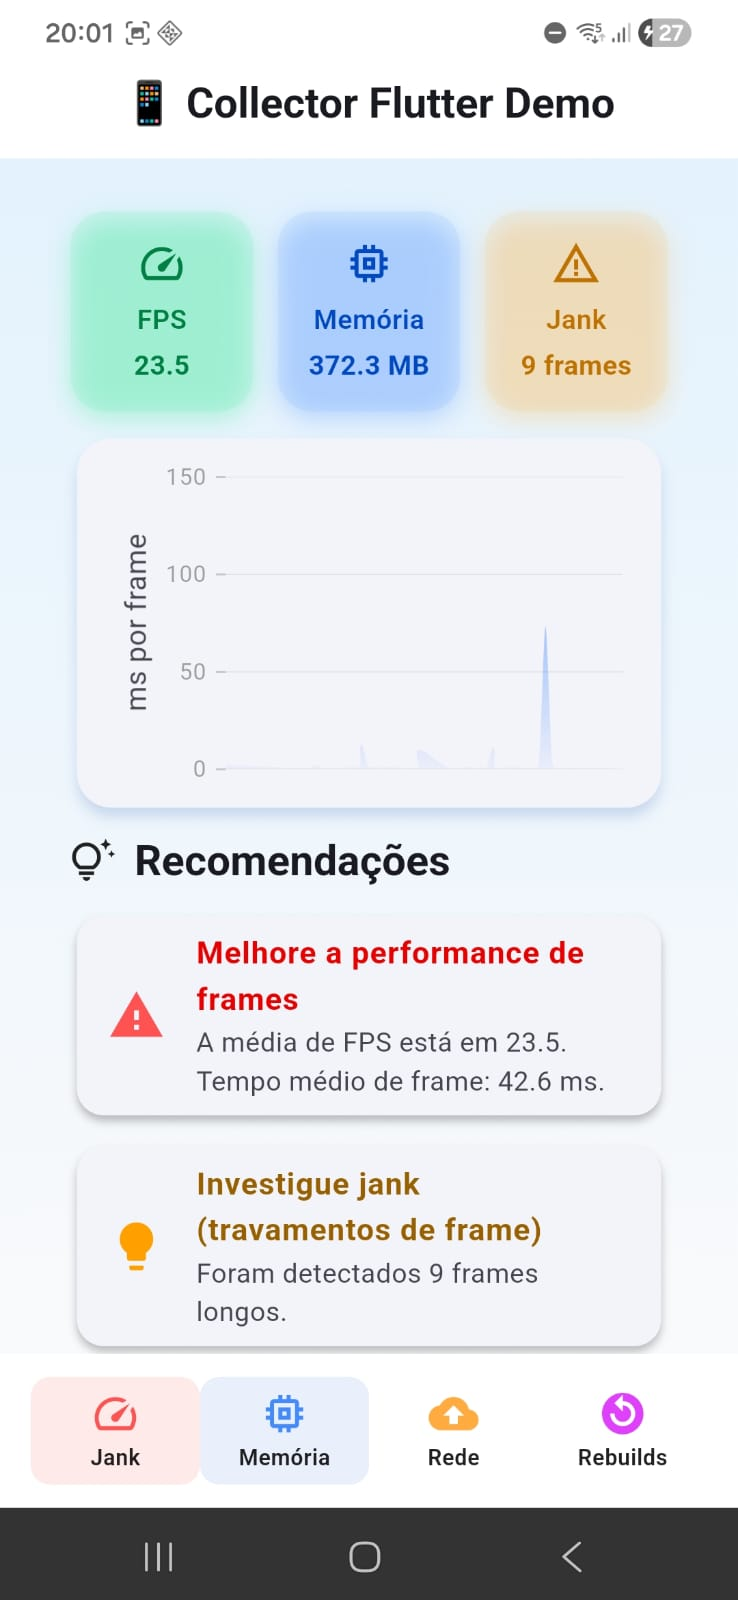
\includegraphics[height=0.8\textwidth]{prototipoquandonaoestaok.jpeg}
  \caption{Painel do aplicativo com anomalias detectadas, como FPS baixo e uso de memória elevado.}
  \label{fig:prototype_notok}
\end{figure}

A Figura~\ref{fig:prototype_icon} identifica o aplicativo de demonstração utilizado nas execuções manuais dos cenários experimentais.

\begin{figure}[H]
  \centering
  
\includegraphics[height=0.3\textwidth]{iconedoappexamplo.jpeg}
  \caption{Ícone do aplicativo de demonstração \texttt{Collector Flutter}.}
  \label{fig:prototype_icon}
\end{figure}


\subsection{Regras de Recomendação}

As recomendações fornecidas pelo módulo \texttt{Recommender} seguem padrões de otimização reconhecidos no ecossistema Flutter e em ferramentas oficiais de diagnóstico~\cite{flutterDevTools2026,android2024}.
Alguns exemplos incluem:

\begin{itemize}
  \item \textbf{Rebuilds frequentes:} “Evite reconstruções excessivas de widgets. Utilize \texttt{const constructors} ou extraia subárvores estáticas.”
  \item \textbf{FPS abaixo de 50:} “Verifique operações pesadas no ciclo de renderização. Considere o uso de \texttt{RepaintBoundary}.”
  \item \textbf{Uso elevado de memória:} “Otimize o descarte de objetos e utilize coleções paginadas.”
  \item \textbf{Chamadas de rede lentas:} “Implemente cache local e controle de tempo de resposta.”
  \item \textbf{Layout sobrecarregado:} “Simplifique hierarquias de widgets e prefira listas com renderização sob demanda, como \texttt{ListView.builder}.”
\end{itemize}

Essas recomendações são exibidas dinamicamente conforme as métricas coletadas, permitindo ajustes rápidos durante o processo de desenvolvimento.

\subsection{Demonstração Prática e Disponibilização do Código-Fonte}

O pacote foi disponibilizado publicamente para garantir transparência e reprodutibilidade dos resultados, conforme recomenda Wohlin \textit{et al.}~\cite{wohlin2012}.

O vídeo de demonstração mostra a execução em tempo real do sistema, com coleta, análise e recomendações heurísticas:

\begin{center}
  \textbf{Acesse o vídeo completo:} \\
  \url{https://drive.google.com/file/d/1KUQ7fFMNRIhe-NSW8loG3wTkQhb_eyOE/view?usp=drive_link}
\end{center}

\noindent
O código-fonte e demais arquivos do projeto estão disponíveis no repositório público:

\begin{center}
  \url{https://github.com/BeatrizVocurcaFrade/collector_flutter}
\end{center}

\noindent
O pacote também foi publicado no repositório oficial do ecossistema Dart/Flutter, permitindo instalação direta e ampliando o acesso da comunidade à ferramenta:

\begin{center}
  \url{https://pub.dev/packages/collector_flutter}
\end{center}

Essa disponibilização em GitHub e pub.dev permite que outros pesquisadores e desenvolvedores avaliem, testem e expandam o sistema, contribuindo para o avanço das pesquisas sobre desempenho e eficiência energética em aplicações Flutter.







% ---------------------------------------------------------------------------------------------------------------------------------------------------------
\section{Critérios de Avaliação}

A validação do pacote \texttt{collector\_flutter} foi conduzida segundo três dimensões efetivamente observadas: \textbf{coerência das métricas coletadas}, \textbf{impacto percebido da coleta} e \textbf{pertinência das recomendações geradas}.
Cada critério foi definido para verificar, de forma funcional, a viabilidade técnica e a aplicabilidade prática do sistema em ambientes reais de desenvolvimento Flutter.



\subsection{Coerência das Métricas Coletadas}

A coerência das métricas foi verificada observando-se se os valores registrados pelo pacote acompanhavam os cenários de carga induzidos no aplicativo de exemplo. Foram analisadas variáveis como tempo médio de renderização de quadros (\textit{frame time}), taxa de quadros por segundo (FPS), consumo de memória, eventos de rede e reconstruções de widgets.

A comparação com ferramentas de referência foi utilizada apenas como apoio qualitativo, sem cálculo formal de erro percentual ou intervalo de confiança. Na versão final documentada, as leituras complementares foram obtidas por \texttt{adb shell dumpsys gfxinfo} e \texttt{adb shell dumpsys meminfo}; Android Profiler e Perfetto permaneceram como referências técnicas do ecossistema, mas não foram empregados como fonte quantitativa de validação.

\subsection{Overhead Introduzido pelo Sistema}

O overhead representa o impacto que o agente de coleta impõe ao desempenho do aplicativo monitorado.
Neste trabalho, esse impacto foi tratado como critério de observação funcional: o coletor deveria permanecer ativo sem impedir a interação com o aplicativo de demonstração nem bloquear a atualização do painel.

Durante os testes, o critério observado foi a manutenção da interação com o aplicativo e da atualização do painel durante a coleta. Não foi realizada mensuração estatística do \textit{overhead}; por isso, os resultados discutem apenas o impacto percebido nas execuções controladas.

\subsection{Eficácia das Recomendações Geradas}

As recomendações heurísticas foram avaliadas verificando-se se o módulo \texttt{Recommender} emitia alertas compatíveis com os gargalos induzidos nos cenários controlados.

Foram analisados sinais como:
\begin{itemize}
  \item \textbf{FPS e \textit{jank}:} recomendações associadas a frames longos e quedas de fluidez;
  \item \textbf{Memória:} alertas relacionados a crescimento sustentado de RSS;
  \item \textbf{Rede:} recomendações diante de volume elevado, falhas ou latência de requisições;
  \item \textbf{Carga combinada:} priorização de recomendações quando múltiplos sintomas ocorrem ao mesmo tempo.
\end{itemize}

\subsection{Clareza da Interface}

A clareza do painel (\texttt{Dashboard}) foi observada por inspeção informal interna durante as execuções manuais, considerando a legibilidade das métricas, a distinção visual dos níveis de severidade e a facilidade de relacionar um alerta ao cenário executado. Essa análise não caracteriza avaliação formal de usabilidade com participantes externos; ela serviu apenas como critério funcional de leitura e interpretação do painel durante os testes.



% ---------------------------------------------------------------------------------------------------------------------------------------------------------



\section{Ferramentas e Ambientes de Desenvolvimento}

O desenvolvimento e a validação do pacote \texttt{collector\_flutter} foram conduzidos em ambiente controlado, com o objetivo de assegurar reprodutibilidade dos resultados e consistência das medições entre diferentes execuções.
As ferramentas selecionadas abrangem IDEs, SDKs e bibliotecas de apoio do ecossistema Flutter, compondo uma infraestrutura moderna, multiplataforma e voltada à análise de desempenho em aplicações Android.

\subsection{Ambientes de Programação e IDEs}

O processo de implementação foi realizado nos seguintes ambientes de desenvolvimento:

\begin{itemize}
  \item \textbf{Visual Studio Code (VS Code):} principal ambiente de escrita e depuração do código Dart e Flutter, configurado com extensões para gerenciamento de pacotes, análise estática e execução de testes unitários.
  \item \textbf{Android Studio:} empregado para execução do aplicativo em dispositivos físicos e emuladores Android, bem como para inspeção complementar de desempenho quando necessário.
\end{itemize}

Ambos os ambientes foram integrados ao controle de versão local via \texttt{Git}, permitindo o gerenciamento seguro e incremental do código-fonte durante o desenvolvimento.

\subsection{SDKs e Dependências Utilizadas}

O ambiente técnico foi configurado com versões estáveis dos SDKs e ferramentas de suporte, garantindo compatibilidade e estabilidade no processo de execução e coleta de métricas:

\begin{itemize}
  \item \textbf{Flutter SDK:} versão \texttt{>=3.22.0} (canal estável), com suporte aos modos \textit{debug}, \textit{profile} e \textit{release}.
  \item \textbf{Dart SDK:} versão correspondente ao Flutter 3.22, utilizada para o desenvolvimento dos módulos de coleta e análise de dados.
  \item \textbf{Android SDK:} configurado com as APIs 33 e 34, compatíveis com Android 12 e 13.
  \item \textbf{Gradle:} atualizado para suportar as dependências do projeto e a integração com o Android Studio.
\end{itemize}

Essa configuração assegura a execução consistente do pacote em diferentes dispositivos Android, com coleta precisa de métricas e comportamento previsível.

\subsection{Ambientes de Teste e Dispositivos}

Os testes experimentais foram realizados exclusivamente em ambiente Android, com dispositivos físicos e emulados representando diferentes capacidades de processamento e arquiteturas.

\begin{itemize}
  \item \textbf{Dispositivos físicos:}
    \begin{itemize}
      \item Samsung Galaxy A52, Android 13;
      \item Motorola G73, Android 12.
    \end{itemize}
  \item \textbf{Emuladores Android:}
    \begin{itemize}
      \item Pixel 6 (x86\_64), Android 14, configurado via Android Studio.
    \end{itemize}
\end{itemize}

Todos os testes foram conduzidos em modo \textit{profile}, permitindo medições precisas de tempo de renderização, FPS e consumo de recursos em condições controladas.

\subsection{Ferramentas de Referência e Validação}

A validação dos resultados obtidos pelo pacote foi realizada com apoio de ferramentas oficiais do ecossistema Android, utilizadas como referência qualitativa para as métricas coletadas:

\begin{itemize}
  \item \textbf{ADB (\textit{Android Debug Bridge}):} empregado para a coleta de informações complementares sobre memória do processo e desempenho de quadros por meio dos comandos \texttt{dumpsys meminfo} e \texttt{dumpsys gfxinfo}.
  \item \textbf{Android Profiler e Perfetto:} utilizados como referências conceituais e ferramentas oficiais de diagnóstico do ecossistema Android, mas sem geração de série comparativa quantitativa neste trabalho.
\end{itemize}

Essas ferramentas apoiaram a interpretação dos resultados, permitindo verificar se os sinais exibidos pelo painel acompanhavam o comportamento esperado dos cenários. A comparação permaneceu qualitativa e não caracteriza medição estatística de precisão.

\subsection{Frameworks e Bibliotecas de Apoio}

Durante o desenvolvimento, foram utilizadas bibliotecas consolidadas do ecossistema Flutter/Dart, responsáveis por facilitar a instrumentação, visualização de dados e controle de estado da aplicação:

\begin{itemize}
  \item \textbf{\texttt{flutter\_bloc}:} gerenciamento reativo de estado, responsável pela comunicação entre coleta, análise e exibição das métricas.
  \item \textbf{\texttt{fl\_chart}:} biblioteca de visualização gráfica utilizada na renderização dos gráficos em tempo real no painel interno (\textit{Dashboard}).
  \item \textbf{\texttt{http}:} responsável pela instrumentação e monitoramento das requisições de rede durante a execução do aplicativo.
  \item \textbf{\texttt{connectivity\_plus}:} monitora eventos de conectividade e simula condições de rede variável.
  \item \textbf{\texttt{logger}:} realiza o registro estruturado de eventos e mensagens internas do sistema, facilitando a depuração.
  \item \textbf{\texttt{vm\_service}:} fornece acesso às APIs internas da máquina virtual Dart, permitindo capturar dados de alocação e uso de memória.
\end{itemize}

Essas dependências foram selecionadas por sua estabilidade, compatibilidade com o ambiente de testes Android e suporte nativo ao desenvolvimento em Dart puro, sem componentes externos.

\subsection{Ambientes de Testes Automatizados}

A confiabilidade do sistema foi verificada por meio de testes unitários e execuções manuais controladas. Essa abordagem garantiu a validação tanto da lógica interna quanto do comportamento visual e interativo do painel.

\begin{itemize}
  \item \textbf{Testes unitários:} implementados com o pacote \texttt{flutter\_test}, abrangendo módulos de coleta e análise (\texttt{Collector}, \texttt{Analyzer} e \texttt{Recommender}).
  Esses testes asseguram que cada componente produza resultados consistentes e corretos em diferentes condições de entrada.
  \item \textbf{Testes manuais:} realizados diretamente em dispositivos físicos e emuladores, com execução de cenários controlados (rebuilds em massa, requisições de rede intensas, simulação de carga de CPU) para observar o comportamento do sistema em tempo real.
\end{itemize}

Essa combinação de testes unitários e manuais possibilitou uma avaliação funcional da coerência das métricas e da estabilidade geral do pacote durante o uso prático.

\vspace{0.5em}

A infraestrutura descrita nesta seção assegura que o pacote \texttt{collector\_flutter} seja executado de forma estável e reproduzível, permitindo uma análise detalhada do desempenho e da eficiência de aplicações Flutter em ambiente Android.
